\documentclass[usenames,dvipsnames]{beamer}
\usepackage{comment}
\usetheme{CambridgeUS}
%\usepackage{macros_gpi}


\usepackage{epsfig}
\usepackage[english]{babel}
\usepackage[utf8]{inputenc}
\usepackage[T1]{fontenc}

\usepackage{appendixnumberbeamer}
\usepackage{epsfig}
\usepackage[english]{babel}
\usepackage[utf8]{inputenc}
\usepackage[T1]{fontenc}
\usepackage{algorithm}
\usepackage{stmaryrd}
%\usepackage{slashbox}
\usepackage{algorithmic}
\usepackage{multirow}   
\usepackage{pstricks}    
\usepackage{color}   
\usepackage{pifont}
\usepackage{supertabular}   
\usepackage{graphicx}
\usepackage{graphbox}
\usepackage{caption}
\usepackage{subcaption}
\usepackage{animate}
%\usepackage{pdfpc-commands}
%\usepackage{xmpmulti}
\captionsetup[figure]{labelformat=empty}
\usepackage{tikz}
\usetikzlibrary{shadows}
\usepackage{fontawesome}
%\newlength{\myheight}

\usepackage{xcolor}
\definecolor{orange-perp}{rgb}{1.0,0.412,0}
\definecolor{prune-saclay}{rgb}{0.388,0,0.235}
\definecolor{bleu-nice}{rgb}{0,0.686,0.843}
\setbeamercolor{author in head/foot}{bg=black,fg=white}
\setbeamercolor{title in head/foot}{fg=black,bg=white}
\setbeamercolor{frametitle}{fg=black,bg=white}
\setbeamercolor{date in head/foot}{bg=black,fg=white}
\setbeamercolor{section in head/foot}{bg=black,fg=white}
\setbeamercolor{subsection in head/foot}{fg=black,bg=white}
\definecolor{darkspringgreen}{rgb}{0.09, 0.45, 0.27}

\setbeamercolor{block body alerted}{bg=white,fg=gray}
\setbeamercolor{block title alerted}{bg=gray,fg=white}

\setbeamercolor{block body}{bg=black!0.2,fg=black}
\setbeamercolor{block title}{bg=black,fg=white}
%\setbeamercolor{block body}{bg=structure!10}
%\setbeamercolor{block title}{bg=structure!20}

\selectlanguage{french}
\setbeamercolor{footlinecolor}{fg=white,bg=black}
\renewcommand\footnoterule{{\color{black}\hrule height 0.5pt width \paperwidth}}

\DeclareMathOperator*{\argmin}{arg\,min\ }


\usepackage{hyperref}
\hypersetup{
  %colorlinks   = true, %Colours links instead of ugly boxes
  %urlcolor     = blue, %Colour for external hyperlinks
  %linkcolor    = blue, %Colour of internal links
  %citecolor   = red %Colour of citations
}

%\setbeamercolor{itemize item}{fg=prune}
%\setbeamercolor{itemize subitem}{fg=prune}
%\setbeamercolor{itemize subsubitem}{fg=prune}

%\setbeamertemplate{itemize item}[ball]{fg=prune}
%\setbeamertemplate{itemize subitem}[ball]{fg=prune}
%\setbeamertemplate{itemize subsubitem}[triangle]

\setbeamercolor{item projected}{fg=white,bg=black}

\setbeamertemplate{itemize item}{%
    \begin{tikzpicture}
        \shade[ball color=black!100!white] (0,0) circle (0.6ex);
    \end{tikzpicture}
}

\setbeamertemplate{itemize subitem}{%
    \begin{tikzpicture}
        \shade[ball color=black!100!white] (0,0) circle (0.6ex);
    \end{tikzpicture}
}


\setbeamercolor*{title}{use=structure,fg=white,bg=black!95}
\setbeamertemplate{title page}[default][colsep=-4bp,rounded=true,shadow=true]
\setbeamertemplate{navigation symbols}{} 
%\setbeamerfont{section number projected}{size=\footnotesize}
%\setbeamercolor{section number projected}{bg=prune,fg=white}
%\setbeamercolor{section in toc}{fg=prune}
%\setbeamercolor{subsection in toc}{fg=prune}
%\setbeamercolor{subsection number projected}{bg=prune}

\setbeamercolor{section number projected}{bg=black,fg=white}
\setbeamercolor{section in toc}{fg=black}
\setbeamercolor{subsection in toc}{fg=black}
\setbeamercolor{subsection number projected}{bg=black}

%\setbeamertemplate{subsections in toc}[square]
\mode<all>

%\setbeamertemplate{footline}{
%\begin{picture}(0,0)(0,0)
%\put(320,4){\footnotesize \insertframenumber{}/\inserttotalframenumber{}}
%\end{picture}
%}
\usepackage{hyperref}
\usepackage{siunitx}

\usepackage{pdfpages}

%\includegraphics[width=1cm]{logo-projet-finance-par-ANR.jpg}

%\title[SKA computing]{\textbf{Le radiotélescope SKA}} 
%\subtitle{Un problème inverse de grande dimension à résoudre en temps réel}

\title[]{\textbf{Problèmes inverses en radioastronomie}\\
\vspace{0.3cm} \textit{Travaux L2S \& SATIE}} 

%\institute{}%Laboratoire des Signaux et Systèmes (L2S) -  Groupe Problèmes Inverses (GPI) }
\author[L2S/SATIE]{
\includegraphics[height=1.7 cm]{logo-saclay-white.png} \\ \vspace{0.5 cm} 
\includegraphics[height=1.7 cm]{L2S_tutelles_vertical.pdf}  \hspace{2cm} 
\includegraphics[height=1.5 cm]{SATIE}
 }
\date[Kick-off ECLAT]{\textit{Labcom ECLAT, Kick-off - 29 juin 2023} }



\begin{document}


%
\includepdf[pages=-]{Slide attente}


\frame[plain]{\titlepage}

%\frame[noframenumbering]{\tableofcontents}
\begin{comment}
%\includegraphics[width=1cm]{logo-projet-finance-par-ANR.jpg}
\title[\textbf{Dark-era project (2021-25)}]{\textbf{Dark-era project}} 
\subtitle{Dataflow Algorithm aRchitecture co-design of SKA pipeline for Exascale Radio Astronomy\\ }
\institute[]{Daniel Charlet$^{**5}$ (IJCLab), Karol Desnos$^{1}$, Mickael Dardaillon$^{3}$, André Ferrari$^{4}$, Chiara Ferrari$^{4}$, Nicolas Gac$^{3}$, Adrien Gougeon$^{2}$, Jean-François Nezan$^{1}$, Nicolas Monnier$^{3}$, François Orieux$^{3}$, Simon Prunet$^{4}$, Martin Quinson$^{2}$, Ophélie Renaud$^{1}$, Frédéric Suter$^{**2}$(IN2P3 Computing Center), Cyril Tasse$^{**5}$ (GEPI), Cédric Viou$^{5}$, Sunrise Wang$^{3\&4}$}
\author[IETR/IRISA/L2S/Lagrange/Nançay]{$^{1}$IETR (INSA),  $^{2}$IRISA (ENS), $^{3}$L2S (CS), $^{4}$Lagrange (UCA),  $^{5}$Nançay (Obs Paris)}
\date[Café sciences CS]{\includegraphics[width=0.25\textwidth]{DARKERA_logo_color.pdf} \hfill
     { \scalebox{0.75}{\tiny{ANR-20-CE46-0001-01} 
\includegraphics[width=0.1\textwidth]{anr-light.pdf}  }} }
\end{comment}

\section{Travaux L2S}

\begin{frame}
  \frametitle{Laboratoire des Signaux et Systèmes (L2S)}
  \vfill %                                                                                                                      
  %Université Paris-Saclay -- CNRS -- CentraleSupélec \vfill
  \vfill
  \begin{block}{Pôle signaux et statistiques}
   \(\approx 30\) permanents et \(\approx30\) doctorants
  \end{block}
  \vfill
  \begin{block}{Travaux en radioastronomie}
    \begin{itemize}
    \item Nicolas Gac \scriptsize{(SATIE au 1$^{er}$ sept. 2023)} \hfill \small{\textit{Adéquation Algorithme Architecture}}
    \item \normalsize{François Orieux} \hfill \small{\textit{Problèmes inverses}}
    \item \normalsize{Mohammed Nabil El Korso} \hfill \small{\textit{Statistiques robustes}}
    \end{itemize}
  \end{block}
  \vfill
  \begin{block}{Thèse Nicolas Monnier (2020-23)}
    \begin{itemize}
        \item \textit{ExaSKA : Parallelization on a High Performance Computing server for the exascale
    radiotelescope SKA}
    \item Collaboration L2S/Obs. Paris/Atos Bull (financement Région IdF)
    \end{itemize}
  \end{block}
\end{frame}

\section{Projet Dark-era}


\subsection{PRC ANR (2021-2025)}
\frame{
%\frametitle{Projet ANR Dark-era}
\begin{block}{Projet ANR Dark-era}
\begin{columns}
\begin{column}{0.5\textwidth}
\includegraphics[width=0.8\textwidth]{DARKERA_logo_color.pdf} 
\end{column}
\begin{column}{0.5\textwidth}
\textit{Dataflow Algorithm aRchitecture co-design of SKA pipeline for Exascale Radio Astronomy}\\
\vspace{0.2cm}
\centering
     { \scalebox{0.75}{\tiny{ANR-20-CE46-0001-01} 
\includegraphics[width=0.4\textwidth]{anr-light.pdf}  }}   
     \end{column}
\end{columns}
\end{block}

\begin{block}{Consortium}
\begin{itemize}
\item \textbf{L2S} \textit{- CentraleSupélec}
\item \textbf{IETR} \textit{- INSA Rennes}
\item \textbf{IRISA} \textit{- ENS Rennes}
\item \textbf{Lagrange} \textit{- Université de la Côte d'Azur}
\item \textbf{Observatoire de Nançay} \textit{- Observatoire de Paris}
\end{itemize}
\end{block}

}

\begin{comment}
\subsection{\textit{SKA computing}, un défi HPC}
\frame{
  %  \frametitle{}
%\scriptsize{

    \begin{block}{Le supercalculateur SDP}
        \begin{itemize}
            \item Très forte \textbf{puissance de calcul} \\ \textit{$\sim 125$ PFLOPS crête (efficacité visée de $\sim$10 $\%$)}   
            \item Traitement en \textbf{temps réel} du flux de données \\\textit{entrée $\sim 8$ Tb/s $\implies$ sortie $\sim 100$ Gb/s}
            \item Budget \textbf{énergétique} limité\\
            \textit{Puissance instantanée $\sim 1 MW$ pour chaque SDP} 
            \item Fossé entre les \textbf{modèles de programmation} utilisés par les astronomes et les développeurs HPC \textit{Python vs MPI/CUDA/...}
        \end{itemize}
       % $\implies$ Challenge to design a power-efficient supercomputer using low power coprocessors for the intensive computing
    \end{block}
    \begin{block}{Défi d'un co-design \textbf{logiciel/matériel}}
       % Need for time and energy performance assessments 
        \begin{itemize}
            \item Chaîne algorithmique en \textbf{flot de donnée} complexe et évolutive
            \item Supercalculateur hétérogène (CPU+GPU) à grande échelle (>100 noeuds) non encore construit
        \end{itemize}
        
        $\implies$ Nécessité d'outils de prototypage rapide pour une \textbf{estimation précoce} des performances en \textbf{temps} et en \textbf{consommation énergétique}
    \end{block}
   
%}
}
\end{comment}

\subsection{Objectifs}
\frame{
  %  \frametitle{}
%\scriptsize{
   
    \begin{block}{Objectifs du projet Dark-era}
        \begin{enumerate}
            \item Construire \textbf{SimSDP, un outil de prototypage rapide} fournissant des simulations \textit{exascale} à partir d'une description en flot de données des algorithmes.
            \item Explorer des \textbf{accélérateurs à basse consommation} alternatifs aux GPUs : FPGA, Kalray MPPA ...
            \item Contribuer au défi calculatoire de SKA
\end{enumerate}
\end{block}
\vspace{0.2cm}
%\centering
    %\frametitle{An interdisciplinary Team}
    %\begin{block}{SimSDP}<2>
        \centering
    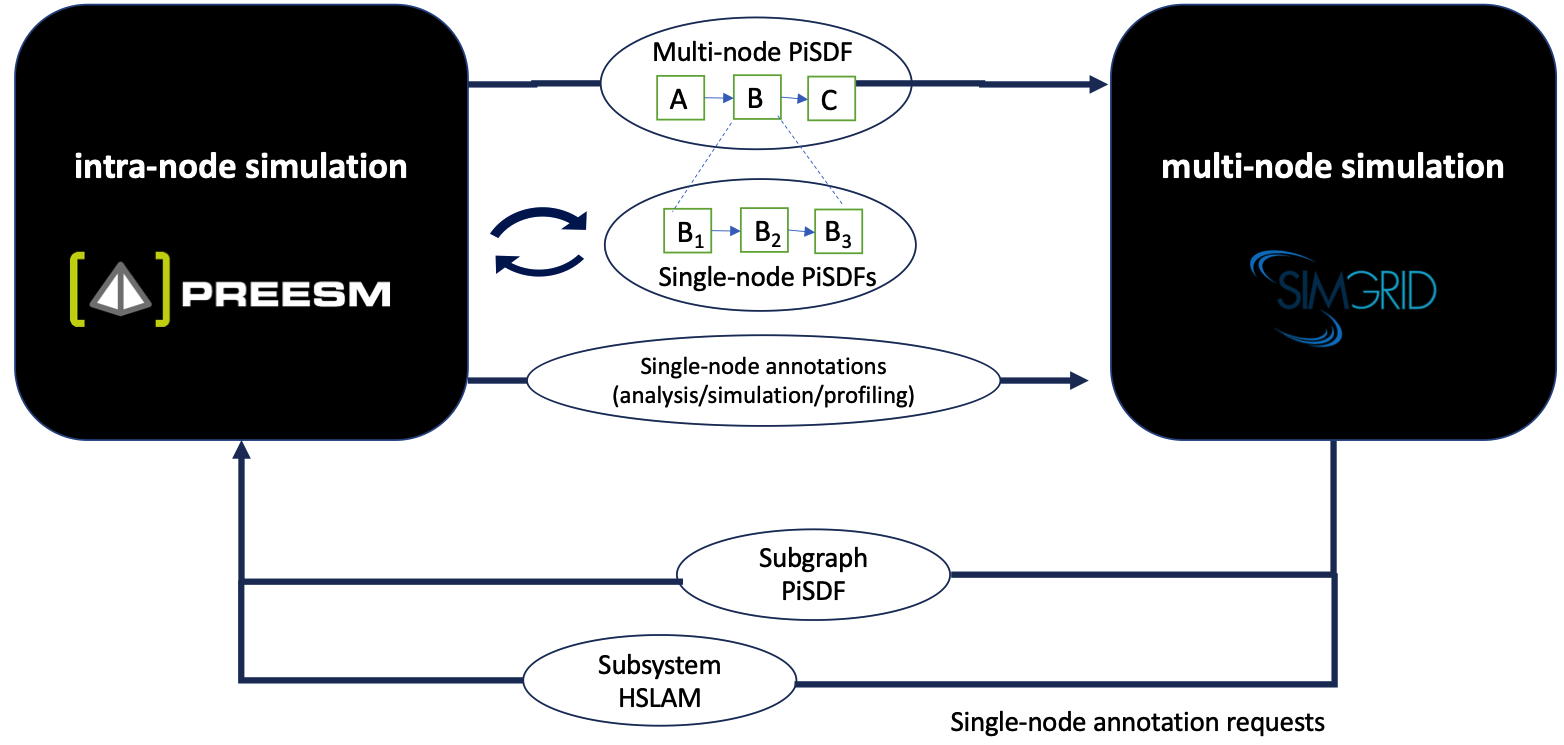
\includegraphics[width=0.7\textwidth]{simsdp_architecture-light.png}  
%\end{block}

}


%The \textbf{SDP supercomputer} will be based on a standard HPC system combined with FPGA or application-specific architectures like GPU or the manycore Kalray Massively Parallel Processor Array (MPPA). One crucial challenge is to assess the performance both in time and energy of new complex scientific \textbf{dataflow algorithms} on not-yet-existing complex computing infrastructures. It will be hardly possible without efficient \textbf{co-design methods} and \textbf{rapid prototyping tools}.




\subsection{Une équipe interdisciplinaire}


\frame{
    %\centering
    %\vspace{0.1cm}
    %
\includegraphics[width=0.2\textwidth]{DARKERA_logo_color_L}  \\
    %\centering
    %\vspace{-0.7cm}
    %\frametitle{An interdisciplinary Team}
    \includegraphics[width=\textwidth]{team_Dark-era.pdf} \\
    
\footnotesize{\textit{Prototypage rapide d’un supercalculateur dédié à la radioastronomie, L’Interdisciplinarité}. \textbf{Voyages au-delà des disciplines, CNRS Edition, 2023}}
}


%Concluion à l'oral sans slide ?
%\subsection{Conclusion}
%\frame{
%\frametitle{Travaux en cours}
%}


\section{Travaux SATIE}

\begin{frame}
  \frametitle{Laboratoire SATIE}
  \vfill %                                                                                                                      
  %Université Paris-Saclay -- CNRS -- CentraleSupélec \vfill
  \vfill
  \begin{block}{Groupe MOSS - Méthodes et Outils pour les Signaux et Systèmes}
    \begin{itemize}
  \item  \(\approx \) 25 permanents et \(\approx\) 20 doctorants
  \item \textbf{Travaux SKA} \\
 \vspace{0.1cm}
  Pascal Larzabal, Lucien Bacharach, Isabelle Vin + Nicolas Gac \scriptsize{(01/09)}
\end{itemize}
  \end{block}
  \vfill

  \begin{block}{Trois thèses en cours}
    \begin{itemize}
     \item \normalsize{Yassine Mhiri (2020-23)}\hfill \scriptsize{Larzabal (SATIE) \& El Korso (L2S)} \\
    \small{\textit{Traitement statistique des signaux observés par les futurs grands radiotélescopes}}\\
    \item \normalsize{Jianhua Wang (2022-25)} \hfill \scriptsize{Larzabal/Bacharach (SATIE) \& El Korso (L2S) } \\
    \small{\textit{Méthodes de traitement du signal pour le design d'instruments en radioastronomie}}\\
    \item \normalsize{Nawel Arab (2022-25)}\hfill \scriptsize{Larzabal (SATIE) \& El Korso (L2S)} \\
    \small{\textit{Maximum de vraisemblance pour l’imagerie dynamique en radioastronomie}}\\
    \end{itemize}
  \end{block}
  
\end{frame}



\section{Travaux futurs}

\begin{frame}
  %\frametitle{Laboratoire SATIE}
  %                                                                                                                      
  %Université Paris-Saclay -- CNRS -- CentraleSupélec \vfill
  \vfill
  \begin{block}{}
    \begin{itemize}
  \item  \(\approx \) 25 permanents et \(\approx\) 20 doctorants
  \item \textbf{Travaux SKA} \\
 \vspace{0.1cm}
  Pascal Larzabal, Lucien Bacharach, Isabelle Vin + Nicolas Gac \scriptsize{(01/09)}
\end{itemize}
  \end{block}
  \vfill

  \begin{block}{Trois thèses en cours}
    \begin{itemize}
     \item \normalsize{Yassine Mhiri (2020-23)}\hfill \scriptsize{Larzabal (SATIE) \& El Korso (L2S)} \\
    \small{\textit{Traitement statistique des signaux observés par les futurs grands radiotélescopes}}\\
    \item \normalsize{Jianhua Wang (2022-25)} \hfill \scriptsize{Larzabal/Bacharach (SATIE) \& El Korso (L2S) } \\
    \small{\textit{Méthodes de traitement du signal pour le design d'instruments en radioastronomie}}\\
    \item \normalsize{Nawel Arab (2022-25)}\hfill \scriptsize{Larzabal (SATIE) \& El Korso (L2S)} \\
    \small{\textit{Maximum de vraisemblance pour l’imagerie dynamique en radioastronomie}}\\
    \end{itemize}
  \end{block}
  
\end{frame}

\setbeamercolor{background canvas}{bg=black}
\section*{C'est fini !}
\frame[t,noframenumbering]
{
  
%\frametitle{Projet ANR DARK-ERA (2/2)}
\vspace{1.1cm}
\centering
{\huge\textcolor{white}{Merci de votre attention }\\
\vspace{1.cm}
\textcolor{white}{\small{\underline{Contacts}}}\\
\flushleft
\normalsize{\textcolor{white}{\textbf{SATIE}}}
\hfill
\normalsize{\textcolor{white}{\textbf{L2S}}}\\
\small{\textcolor{white}{nicolas.gac@universite-paris-saclay.fr}
\hfill
\textcolor{white}{francois.orieux@l2s.centralesupelec.fr}\\
\hfill
\textcolor{white}{mohammed.nabil.el-korso@l2s.centralesupelec.fr}}\\
\vspace{1cm}
\textcolor{white}{\small{\underline{Site web Dark-era}} : \href{https://dark-era.pages.centralesupelec.fr}{\textcolor{white}{https://dark-era.pages.centralesupelec.fr}}}}\\
%\vspace{0.5cm}
\textcolor{white}{\small{\underline{Fête de la science} : \href{https://www.youtube.com/watch?v=ro2mqx5QQnI&feature=youtu.be}{\tiny{\textcolor{white}{https://www.youtube.com/watch?v=ro2mqx5QQnI\&feature=youtu.be}}}}}\\

}



\appendix
\section*{Post traitement}
\setbeamercolor{background canvas}{bg=white}
\frame{
\begin{block}{Séparation de source pour le démélange de gaz interstellaires}
      \begin{minipage}[htb]{0.4\linewidth}
      \centering
  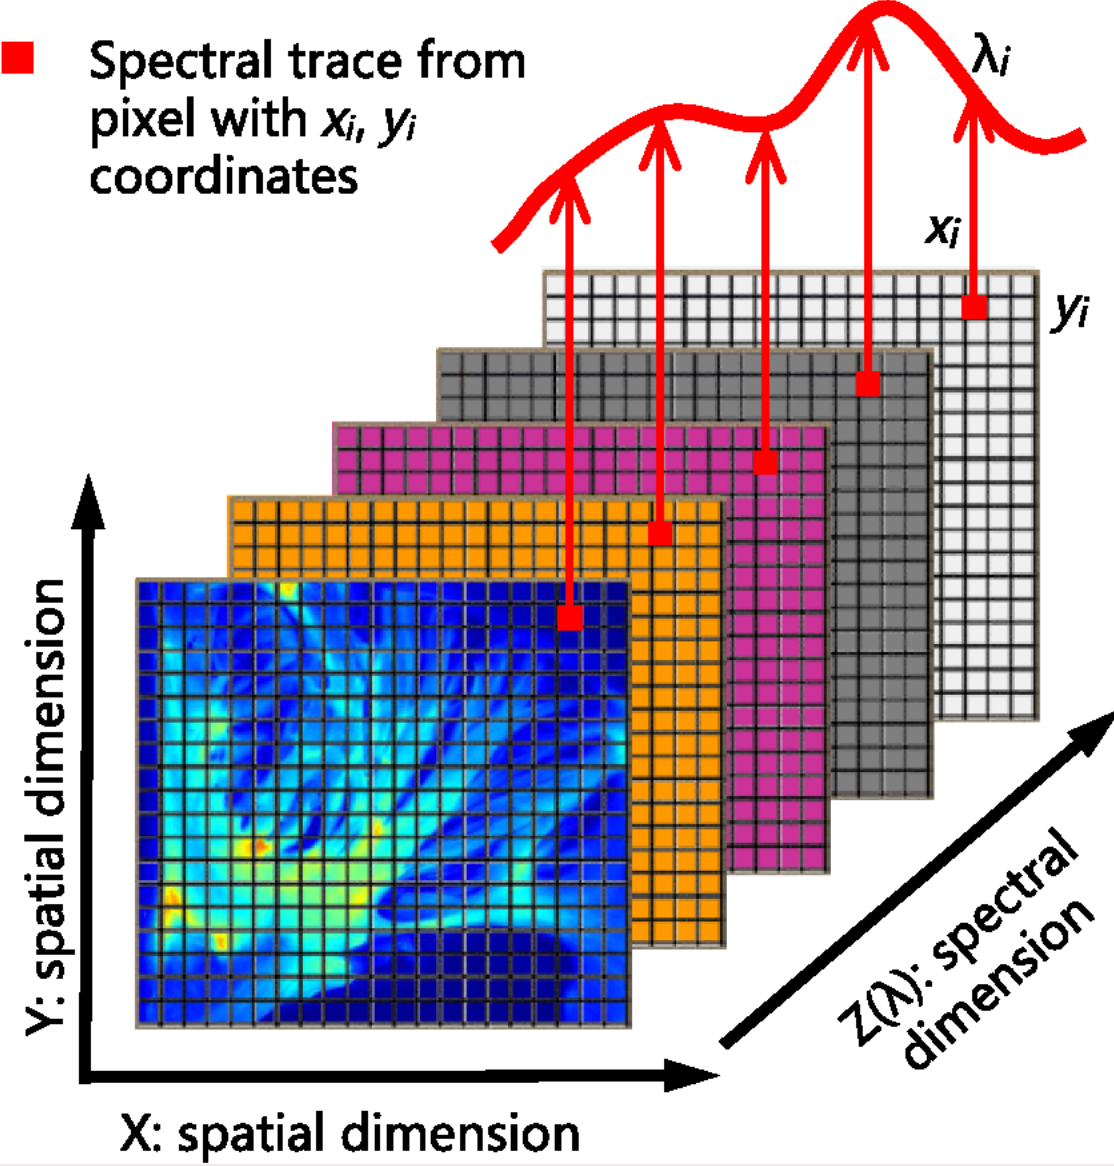
\includegraphics[height=4cm]{hypercube}
  \end{minipage}
  \begin{minipage}[htb]{0.59\linewidth}
      \centering
      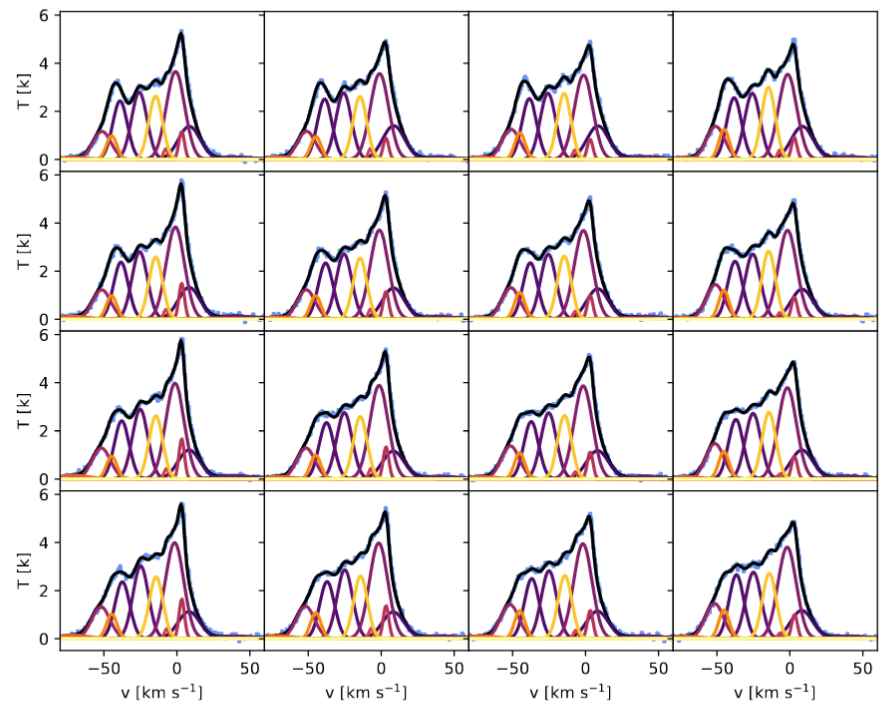
\includegraphics[height=4cm]{courbes.png}\\
  \end{minipage}\\
  \vspace{0.5cm}
  \textit{Projet CNRS HyperStars avec CEA-Irfu/LIP6 (M.A. Miville-Deschênes)} 
  \end{block}
}
\end{document}

